\documentclass[
  man,
  longtable,
  nolmodern,
  notxfonts,
  notimes,
  colorlinks=true,linkcolor=blue,citecolor=blue,urlcolor=blue]{apa7}

\usepackage{amsmath}
\usepackage{amssymb}




\RequirePackage{longtable}
% \setlength\LTleft{0pt}
\RequirePackage{threeparttablex}

% % % \RequirePackage{rotating}
% \RequirePackage{threeparttablex}
% \DeclareDelayedFloatFlavor{sidewaysfigure}{figure}
% \DeclareDelayedFloatFlavor{sidewaystable}{table}
% \DeclareDelayedFloatFlavor{longtable}{table}
\DeclareDelayedFloatFlavor{ThreePartTable}{table}


% % 


\makeatletter
\renewcommand{\paragraph}{\@startsection{paragraph}{4}{\parindent}%
	{0\baselineskip \@plus 0.2ex \@minus 0.2ex}%
	{-.5em}%
	{\normalfont\normalsize\bfseries\typesectitle}}

\renewcommand{\subparagraph}[1]{\@startsection{subparagraph}{5}{0.5em}%
	{0\baselineskip \@plus 0.2ex \@minus 0.2ex}%
	{-\z@\relax}%
	{\normalfont\normalsize\bfseries\itshape\hspace{\parindent}{#1}\textit{\addperi}}{\relax}}
\makeatother




\usepackage{longtable, booktabs, multirow, multicol, colortbl, hhline, caption, array, float, xpatch}
\setcounter{topnumber}{2}
\setcounter{bottomnumber}{2}
\setcounter{totalnumber}{4}
\renewcommand{\topfraction}{0.85}
\renewcommand{\bottomfraction}{0.85}
\renewcommand{\textfraction}{0.15}
\renewcommand{\floatpagefraction}{0.7}

\usepackage{tcolorbox}
\tcbuselibrary{listings,theorems, breakable, skins}
\usepackage{fontawesome5}

\definecolor{quarto-callout-color}{HTML}{909090}
\definecolor{quarto-callout-note-color}{HTML}{0758E5}
\definecolor{quarto-callout-important-color}{HTML}{CC1914}
\definecolor{quarto-callout-warning-color}{HTML}{EB9113}
\definecolor{quarto-callout-tip-color}{HTML}{00A047}
\definecolor{quarto-callout-caution-color}{HTML}{FC5300}
\definecolor{quarto-callout-color-frame}{HTML}{ACACAC}
\definecolor{quarto-callout-note-color-frame}{HTML}{4582EC}
\definecolor{quarto-callout-important-color-frame}{HTML}{D9534F}
\definecolor{quarto-callout-warning-color-frame}{HTML}{F0AD4E}
\definecolor{quarto-callout-tip-color-frame}{HTML}{02B875}
\definecolor{quarto-callout-caution-color-frame}{HTML}{FD7E14}

\newlength\Oldarrayrulewidth
\newlength\Oldtabcolsep


\usepackage{hyperref}




\providecommand{\tightlist}{%
  \setlength{\itemsep}{0pt}\setlength{\parskip}{0pt}}
\usepackage{longtable,booktabs,array}
\usepackage{calc} % for calculating minipage widths
% Correct order of tables after \paragraph or \subparagraph
\usepackage{etoolbox}
\makeatletter
\patchcmd\longtable{\par}{\if@noskipsec\mbox{}\fi\par}{}{}
\makeatother
% Allow footnotes in longtable head/foot
\IfFileExists{footnotehyper.sty}{\usepackage{footnotehyper}}{\usepackage{footnote}}
\makesavenoteenv{longtable}

\usepackage{graphicx}
\makeatletter
\def\maxwidth{\ifdim\Gin@nat@width>\linewidth\linewidth\else\Gin@nat@width\fi}
\def\maxheight{\ifdim\Gin@nat@height>\textheight\textheight\else\Gin@nat@height\fi}
\makeatother
% Scale images if necessary, so that they will not overflow the page
% margins by default, and it is still possible to overwrite the defaults
% using explicit options in \includegraphics[width, height, ...]{}
\setkeys{Gin}{width=\maxwidth,height=\maxheight,keepaspectratio}
% Set default figure placement to htbp
\makeatletter
\def\fps@figure{htbp}
\makeatother


% definitions for citeproc citations
\NewDocumentCommand\citeproctext{}{}
\NewDocumentCommand\citeproc{mm}{%
  \begingroup\def\citeproctext{#2}\cite{#1}\endgroup}
\makeatletter
 % allow citations to break across lines
 \let\@cite@ofmt\@firstofone
 % avoid brackets around text for \cite:
 \def\@biblabel#1{}
 \def\@cite#1#2{{#1\if@tempswa , #2\fi}}
\makeatother
\newlength{\cslhangindent}
\setlength{\cslhangindent}{1.5em}
\newlength{\csllabelwidth}
\setlength{\csllabelwidth}{3em}
\newenvironment{CSLReferences}[2] % #1 hanging-indent, #2 entry-spacing
 {\begin{list}{}{%
  \setlength{\itemindent}{0pt}
  \setlength{\leftmargin}{0pt}
  \setlength{\parsep}{0pt}
  % turn on hanging indent if param 1 is 1
  \ifodd #1
   \setlength{\leftmargin}{\cslhangindent}
   \setlength{\itemindent}{-1\cslhangindent}
  \fi
  % set entry spacing
  \setlength{\itemsep}{#2\baselineskip}}}
 {\end{list}}
\usepackage{calc}
\newcommand{\CSLBlock}[1]{\hfill\break\parbox[t]{\linewidth}{\strut\ignorespaces#1\strut}}
\newcommand{\CSLLeftMargin}[1]{\parbox[t]{\csllabelwidth}{\strut#1\strut}}
\newcommand{\CSLRightInline}[1]{\parbox[t]{\linewidth - \csllabelwidth}{\strut#1\strut}}
\newcommand{\CSLIndent}[1]{\hspace{\cslhangindent}#1}





\usepackage{newtx}

\defaultfontfeatures{Scale=MatchLowercase}
\defaultfontfeatures[\rmfamily]{Ligatures=TeX,Scale=1}





\title{The Impact of Response Options on Gender Categorization of Faces}
\shorttitle{The Impact of Response Options on Gender Categorization of
Faces}


\usepackage{etoolbox}





\author{Elli van Berlekom}


\affiliation{
{Psychology, Stockholm University}}






\leftheader{Berlekom}


\date{2024-04-23}

\abstract{Gender is not a binary category, yet much of gender
categorization research continues to treat it as such in terms of
response options. This study comprises two experiments that challenge
the binary gender norm by exploring alternative response options to
measure gender categorization. In Experiment 1 (N=66), we compared
one-dimensional and two-dimensional scales for gender categorization of
a diverse set of morphed faces. We found that regardless of the response
options used, participants treated gender categorically. In other words,
participants accentuated their categorizations of womanhood and manhood,
even when response options did not frame them as opposites. In
Experiment 2 (N = 105) we compared traditional binary response options
with multiple categories and free-text answers. The results suggested
that while non-binary options such as ``non-binary'' and ``I don't
know'' led to categorizations beyond the binary framework in about half
of the participants, free-text options did not elicit similar results.
Despite the opportunity to categorize faces beyond the binary, the
predominant categorizations remained as `woman' or `man'. We conclude
that while inclusive response options can facilitate acknowledgment of
gender diversity, they do not fundamentally alter the binary perception
of gender.}
% 


\authornote{\par{\addORCIDlink{Elli van Berlekom}{0000-0002-8393-5316}}
\par{ }
\par{       }
\par{Correspondence concerning this article should be addressed to Elli
van Berlekom, Email: elli.vanberlekom@psychology.su.se}
}


\makeatletter
\let\endoldlt\endlongtable
\def\endlongtable{
\hline
\endoldlt
}
\makeatother
\RequirePackage{longtable}
\DeclareDelayedFloatFlavor{longtable}{table}
% \RequirePackage{threeparttablex}
% \DeclareDelayedFloatFlavor{ThreePartTable}{table}

\urlstyle{same}



% From https://tex.stackexchange.com/a/645996/211326
%%% apa7 doesn't want to add appendix section titles in the toc
%%% let's make it do it
\makeatletter
\xpatchcmd{\appendix}
  {\par}
  {\addcontentsline{toc}{section}{\@currentlabelname}\par}
  {}{}
\makeatother

\begin{document}

\maketitle


\setcounter{secnumdepth}{-\maxdimen} % remove section numbering

\setlength\LTleft{0pt}




Many transgender and nonbinary (TNB) people experience gender as
flexible, fluid, diffuse, and not bounded by the typical binary of women
and men (Hyde et al., 2018; Richards et al., 2016). Unlike cisgender
people - who identify with their assigned sex at birth - transgender
people identify with a gender different from their assigned sex at birth
(Levitt \& Ippolito, 2014). Moreover, many transgender people identify
as nonbinary, which can be either an identity in and of itself or an
umbrella term for a wide variety of gender identities other than woman
or man (e.g.~genderqueer, agender, genderfluid) (Monro, 2019).

In surveys and questionnaires that measure gender identity, however,
gender has traditionally been constructed as a binary, where response
options are limited to the categories of woman/female and man/male
(Saperstein \& Westbrook, 2021). Such measurement invisibilizes and
implicitly delegitimizes TGD identities (Ansara \& Hegarty, 2014).
Recently, psychologists have been encouraged to include a wider range of
response options (Saperstein \& Westbrook, 2021) or use free text
options (Lindqvist et al., 2020). As awareness of gender diversity is
increasing, these practices are becoming more common (see Carleton et
al., 2022; Cronin et al., 2022; D'Agostino et al., 2022 for some recent
examples). Research on gender categorization of others, however, is
still dominated by binary response options (eg. Campanella et al., 2001;
Habibi \& Khurana, 2012; Jung et al., 2019). Here we report two studies
demonstrating how gender categorization of faces can be measured without
reinforcing binary gender norms.

\subsection{Two Challenges to the Gender
Binary}\label{two-challenges-to-the-gender-binary}

An early challenge to the norm of binary measurement of gender in
psychology came from Sandra Bem in the ´70s (Bem, 1974). She devised a
scale that measured gender as a psychological trait, treating femininity
and masculinity as two separate constructs. This scale allowed for
combinations of gender which challenged previous binary conceptions.
Such combinations included ``androgynous'', which meant scoring high on
both femininity and masculinity; and agender, which meant scoring low on
both. Characteristically for research of its time, Bem still largely
accepted the binary gender framework. In treating gender as a
psychological trait, for example, the BSRI implicitly assumed all
respondents were women or men.

A later group of challenges to the gender binary in psychology emerged
in the 2010s and onward. These researchers, often drawing from feminist
and queer scholarship (e.g. Butler, 1999), were explicit about the need
for psychology to include trans and non-binary gender identities (Hyde
et al., 2018; Morgenroth \& Ryan, 2018; Richards et al., 2016).
Saperstein and Westbrook (2021), for example, suggested that surveys
measuring gender include a range of response options, such as
non-binary, other, trans man, agender, and more. Lindqvist et al. (2020)
suggested an open text entry where participants can fill in their gender
in an open-ended format. The free text response has the advantage of
being completely unconstrained, allowing participants to enter any
category, including categories which may not have occurred to the
researchers. Moreover, the acceptable terms sometimes shift over time,
as more marginalized voices are heard. The term ``transsexual'' for
example, has been widely used and seen as acceptable, but is now
understood to be stigmatizing (APA manual). A free text avoids this
issue.

Both the initial and later challenges to the gender binary in psychology
primarily suggested ways to measure respondents' own gender identity.
This emphasis is understandable as gender identity is a commonly
reported demographic variable. But gender is frequently also measured in
terms of participants' categorizations of others. Because
self-categorization and categorization of others are different
processes, however, the best measurement of self-categorization may not
be the best measurement of the categorization of others.

\subsection{Measuring gender categorization of
others}\label{measuring-gender-categorization-of-others}

Research on how people perceive and categorize the gender of others has
used both dimensional scales as well as discrete categories, but in both
cases almost exclusively treats gender as a binary category. It is
fairly common, for example, to use the one-dimensional approach, where
participants rate the gender of others as a single dimension, from
masculine to feminine. Much of this research explores evolutionary and
other reasons for gender in faces, correlating one-dimensional
categorization of facial gender with other traits, such as
attractiveness (Little \& Hancock, 2002), and distinctiveness (O'Toole
et al., 1998).

Another common approach tasks people to categorize faces according to a
set of response options decided by the researchers, almost invariably
``woman'' and ``man''. Studies using this method have shown that people
rapidly and automatically categorize gender (Habibi \& Khurana, 2012;
Jung et al., 2019). This, in turn, indicates that gender is a salient
category that determines how people evaluate others on traits, such as
agreeableness, dominance, etc (Stolier \& Freeman, 2017).

Moreover, participants categorize faces categorically (Campanella et
al., 2001). This phenomenon has been observed when participants
categorize faces that have been morphed to vary from feminine to
masculine. Categorizations of these morphed faces were accentuated so
that for example a 60\% female morph was rated as a woman by close to
80\% of participants (Campanella et al., 2001). Observing categorical
effects for any stimuli suggests that people treat that stimuli as two
separate categories (Simanova et al., 2016). The observation of a
categorical effect for gender suggests that people think of gender as a
strict binary consisting of women and men only.

However, this research has rarely considered the risk that the structure
of response options could communicate certain ideas about gender to
participants. A one-dimensional scale implies that gender can vary on a
continuum. It also places masculinity and femininity at the endpoints of
the scales, so that a higher rating of femininity is by definition a
lower rating of masculinity. This in turn suggests that someone cannot
embody femininity and masculinity at the same time, indeed, that the two
concepts are opposites. Binary response options consisting of
woman/female and man/male only suggest that those are the only two
categories that exist. On the other hand, two-dimensional scales and
categories that include non-binary response options suggest the
opposite, that femininity and masculinity are not mutually exclusive and
that a multiplicity of genders exists. In other words, no matter which
type of response options are used, ideas are being communicated to
participants, potentially influencing their responses. Most
recommendations suggest taking great care not to influence participants
(Nichols \& Maner, 2008), but the effects of gender response options are
rarely considered.

Another aspect of gender categorizations of others is that complete
certainty is not possible. This is because many trans and non-binary
individuals do not have a prototypical androgynous gender expression
(Richards et al., 2016). Indeed many non-binary and even binary trans
people may appear similar to their assigned gender at birth. Therefore,
if a person aims to be inclusive, abstaining from categorizing until
more information is available is always the safest option when
encountering a face. However, this aspect of gender categorization has
received very little attention from researchers.

The purpose of Study 1 was to investigate the influencing effect of one
and two-dimensional response options by investigating whether
participants' responses are categorical. A categorical effect is a
useful outcome in this context because it suggests participants treat
gender as consisting of only two categories: women and men. Drawing
inspiration from Bem (1974) we compare gender categorization measured
using one-dimensional response options and two-dimensional response
options. If one-dimensional scales influence participants to think of
gender as binary and opposites and two-dimensional scales don't do this,
there should be a reduced categorical effect for two-dimensional scales.
We tested two research questions; would participants respond
categorically to faces (Research Question 1) and would a one-dimensional
rating scale elicit stronger categorical responses than two-dimensional
(Research Question 2)?

The purpose of Study 2 was to investigate categorization using
non-binary gender response options. We included multiple categories
beyond women and men, as suggested by for example Saperstein and
Westbrook (2021) and we also included a free text as suggested by
Lindqvist and colleagues (2019) Study 2 was mainly interested in how the
two non-binary options compared to each other and how the presence of
non-binary options affected the categorization of binary gender. As
non-binary options have been promoted by feminist and LGBTQ+ activists,
their inclusion might have more generalized effects on binary
categorization. Therefore, study 2 also investigated the categorization
of women and men.

\section{Study 1}\label{study-1}

\subsection{Method}\label{method}

\subsubsection{Participants}\label{participants}

Swedish participants (\emph{N} = 66) took part in the study in a lab at
a Stockholm University campus (\emph{M}\textsubscript{age}= 37.36,
\emph{SD}\textsubscript{age} = 14.14, Range = 18 - 73). Self-identified
gender was measured using an open-ended text box (33 women, 35 men, and
2 participants who did not indicate gender). Participants were
monetarily compensated for their time (100 sek). All participants were
informed that participation was voluntary and gave written consent to
participate in the study.

\subsubsection{Stimuli}\label{stimuli}

The experiment included Black, Asian, and White faces from the London
Face Database (L. M. DeBruine \& Jones, 2017)and the Chicago Face
Database(Ma et al., 2015) morphed with Webmorph (L. DeBruine, 2018). We
matched the faces of women and men using the codebook provided by the
researchers, ensuring that the women were rated similar levels of
feminine as the men were rated masculine. The morphs were made in 7
steps, from completely feminine to completely masculine. We defined the
facial gender as the degree of the female face present in the morph. In
other words, a 33\% face was slightly tilted toward the man, a 50\% face
was an even mixture and a 100\% face consisted only of the woman's face.
Because there were 18 pairs morphed in 7 steps, the total number of
faces was 126.

\begin{figure}

\caption{\label{fig-stimuli}Example of a seven-step morphing spectrum}

\centering{

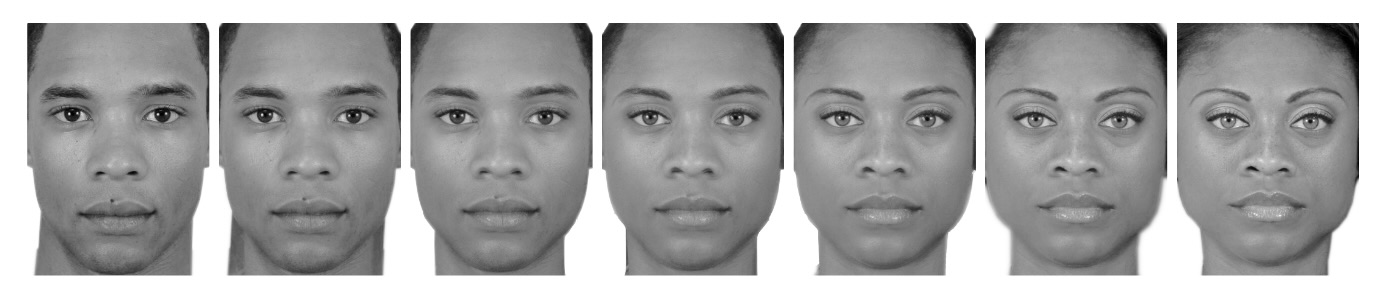
\includegraphics{pix/stimuli.jpeg}

}

\end{figure}%

\subsubsection{Design and procedure}\label{design-and-procedure}

The experiment used a between-participants design. The two conditions
were the \emph{one-dimensional} (control condition), and
\emph{two-dimensional} (experimental) conditions. Participants were
randomly allocated into one of the two response option conditions
(\emph{N}\textsubscript{1d} = 28, \emph{N}\textsubscript{2d} = 38).

Participants completed the experiment on a computer in a quiet room.
Each trial consisted of a face accompanied by the question ``How would
you gender categorize this person?''. In the one-dimensional control
condition, participants rated gender based on a single continuum with
the anchors marked ``woman'' and ``man''. In the two-dimensional
condition, participants rated each face twice on two different continua,
in the ``woman'' continuum, the anchors were marked ``not woman'' and
``woman''; in the ``man'' continuum the anchors were marked ``not man''
and ``man''. The separate continua were presented on different trials
and the order of trials was completely randomized (see
Figure~\ref{fig-exp2-trial}).

\begin{figure}

\caption{\label{fig-exp2-trial}Sample trial from each of the three
conditions}

\centering{

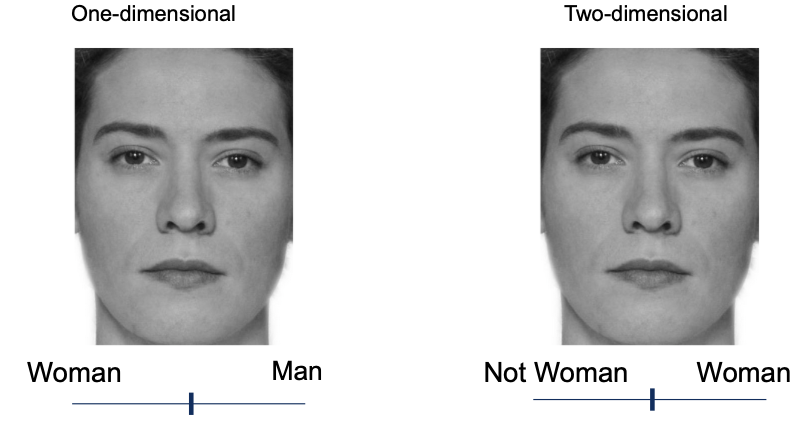
\includegraphics{pix/exp2.png}

}

\end{figure}%

\subsubsection{Data analysis}\label{data-analysis}

We used R (Version 4.2.2; R Core Team, 2022) and the R-packages
\emph{brms} (Version 2.18.0; Bürkner, 2017, 2018, 2021), \emph{papaja}
(Version 0.1.1; Aust \& Barth, 2022), and \emph{tidyverse} (Version
1.3.2; Wickham et al., 2019). We fit the data to Bayesian mixed-effects
models to test the categorical effects. In all models, morph level and
response options were included as fixed effects. Additionally, all
models included varying intercepts for both participants and trials and
varying slopes for facial gender. The pattern of scores was non-linear,
meaning any linear model would probably be misspecified. Therefore, to
reduce the complexity of the model, facial femininity was modeled as an
ordered factor with seven levels, corresponding to each of the seven
morphing steps.

\subsection{Results}\label{results}

\subsubsection{Participant flow}\label{participant-flow}

All participants completed the experiment and were included in the
analyses. The one-dimension condition included 28 participants and the
two-dimension condition included 38 participants.

\subsubsection{Descriptive statistics}\label{descriptive-statistics}

First, we examined the relationship between ratings of ``woman'' and
``man'' in the multiple dimensions condition. These were highly
correlated (R = 0.86). Second, we examined whether participants
responded categorically to faces (Research Question 1). Individual-level
(thin lines) and group mean (thick lines) responses are visualized in
Figure Figure~\ref{fig-desc-two}. If participants respond only to the
morph of faces, the lines should be a straight diagonal. Instead,
Figure~\ref{fig-desc-two} shows that most participants display a
non-linear S-shape and this was also the pattern of the group means.

\begin{figure}

\caption{\label{fig-desc-two}Participant level and mean ratings of faces
in One-dimensiona and two-dimensional conditions}

\centering{

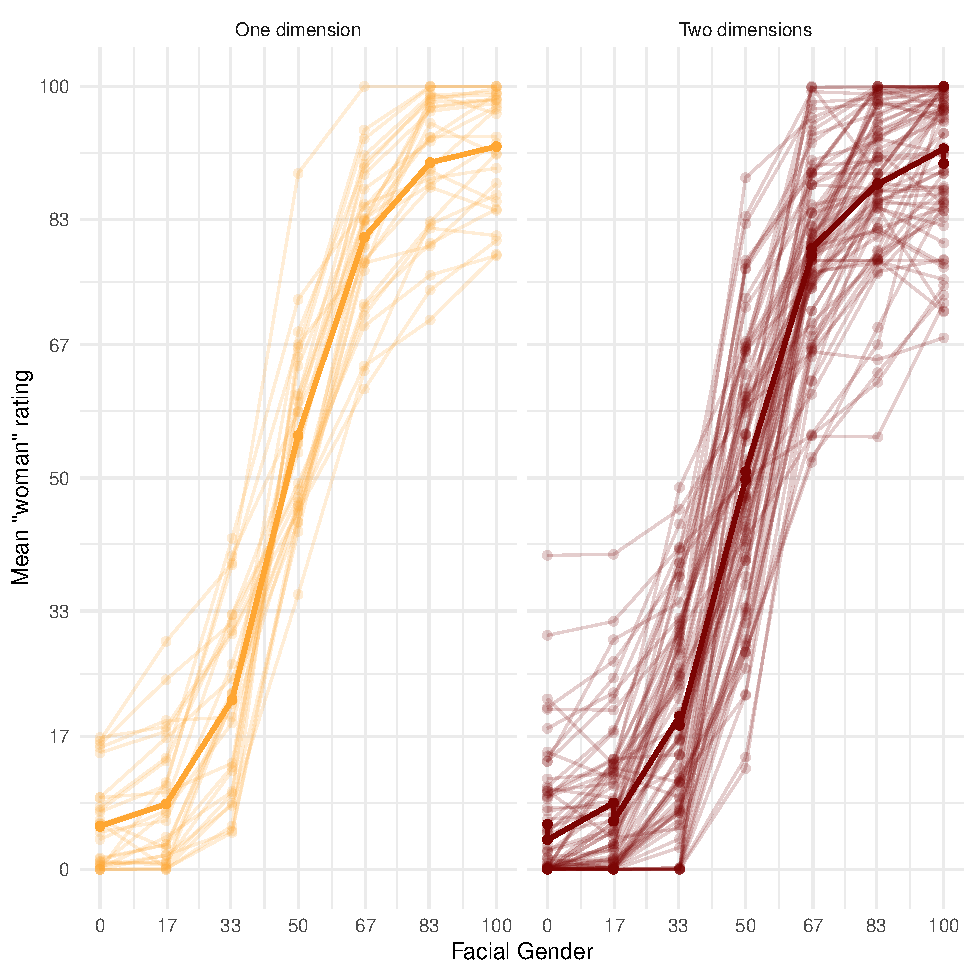
\includegraphics{quarto_test_files/figure-pdf/fig-desc-two-1.pdf}

}

\end{figure}%

\subsubsection{Inferential Statistics}\label{inferential-statistics}

To further test this, we calculated the difference between the mean
ratings when facial gender was 33 and 67. If participants respond
linearly, this difference should be 34. Instead, in both the
one-dimensional condition (\emph{M}\textsubscript{1D} = 59.58,
CI\textsubscript{1D} = {[}53.65, 65.26{]}) and the two-dimensional
condition (\emph{M}\textsubscript{2D} = 58.75, CI = {[}53.65, 65.26{]})
this difference far exceeded 34 and the narrow credible intervals
suggest these measures were precisely estimated. We interpret this to
mean that participants responded categorically. However, Figure 3 also
suggests that there was a degree of individual variation, and some
participants were more categorical than others in their ratings.

Finally, we tested whether the categorical perception was reduced in the
two-dimension condition compared to the one-dimension condition
(Research Question 2). The two conditions were not meaningfully
different (Difference = -0.83, CI = {[}-5.57, 7.24{]},
BF\textsubscript{01}= 30.47). This suggests that categorical perception
was not reduced by two-dimensional response options.

\subsection{Discussion}\label{discussion}

Participants responded categorically when rating faces in terms of
gender. Additionally, two-dimensional response options did not reduce
this effect. Indeed a highly binary view of gender was present and
participants treated womanhood and manhood as opposites even though the
scale would allow them to be more flexible. However, this scale only
implicitly challenged the binary, as no diverse gender options were
present.

\section{Study 2}\label{study-2}

Study 2 tested a wider range of response options that explicitly
challenge the gender binary. These were adapted from common ways to
measure participants' self-categorization of gender (Lindqvist et al.,
2020; Saperstein \& Westbrook, 2021). Study 2 compared a control
condition consisting of standard binary response options to two
alternatives: a third gender option (such as `non-binary' or `other')
and an open text box for participants to type in their response.

\subsection{Method}\label{method-1}

\subsubsection{Participants}\label{participants-1}

Swedish participants (\emph{N} = 66) took part in the study in a lab at
a Stockholm University campus (\emph{M}\textsubscript{age}= 37.36,
\emph{SD}\textsubscript{age} = 14.14, Range = 18 - 73). Self-identified
gender was measured using an open-ended text box as recommended by
(Lindqvist et al., 2020) (56 women, 47 men 2 participants did not
indicate gender). All participants were informed that participation was
voluntary and gave written consent to participate in the study.

\subsubsection{Stimuli}\label{stimuli-1}

The stimuli were identical to those of Study 1. In short, the stimuli
comprised a multiracial set of faces morphed to vary in terms of facial
gender. We defined facial gender as the degree of the female face
present in the morph. In other words, a 33 face was slightly tilted
toward the man, a 50 face was an even mixture and a 100 consisted only
of the woman's face. Because there were 18 pairs morphed in 7 steps, the
total number of faces was 126.

\subsubsection{Design and Procedure}\label{design-and-procedure-1}

The experiment used a between-participants design. There were three
response options conditions: \emph{binary categories}, \emph{free text},
and \emph{multiple categories} (see Figure~\ref{fig-exp1-trial}). In the
binary categories condition, the response options consisted of two
categories: ``woman'' and ``man''. In the free text condition, the
response options consisted of an open text box. In the multiple
categories condition, the response options consisted of four categories:
``woman'', ``man'', ``other'' and ``I don't know''.

Participants completed the experiment on a computer in a quiet room.
Each trial consisted of a face accompanied by the question ``How would
you gender categorize this person?'' After being allocated to one of the
three conditions, participants categorized 126 faces according to the
response options in their condition.

\begin{figure}

\caption{\label{fig-exp1-trial}Sample trial from each of the three
conditions}

\centering{

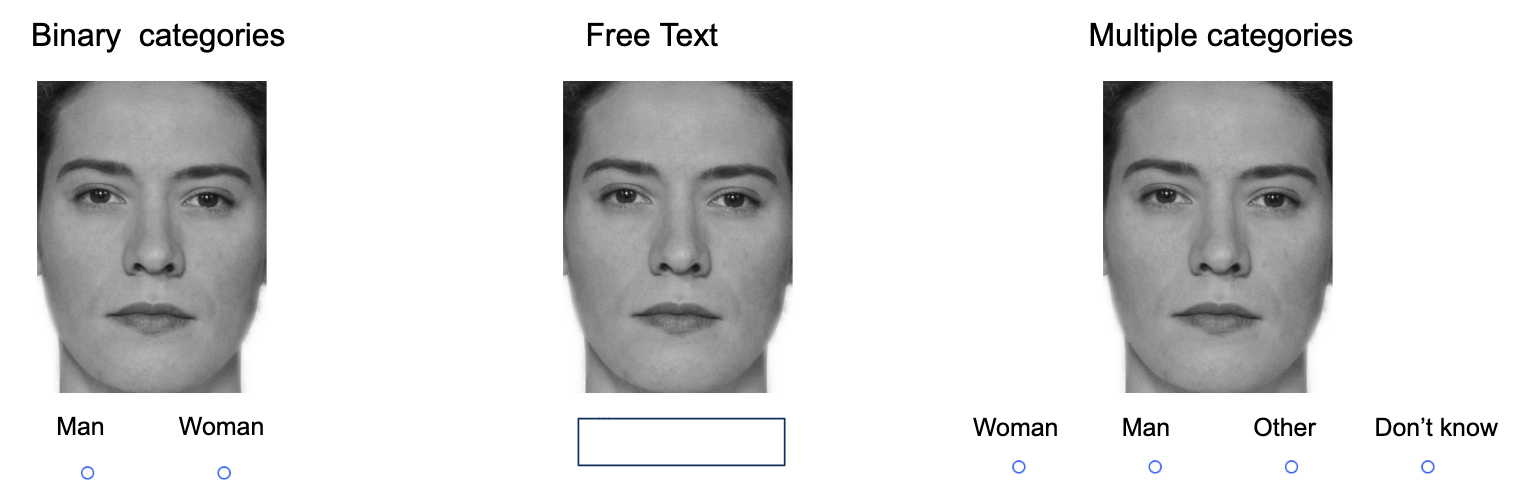
\includegraphics{pix/exp1.png}

}

\end{figure}%

The outcome was responses to the categorization task. For analysis
purposes, these were aggregated in the following ways:

\emph{Other categorizations} represented the trials where participants
categorized faces as any other category than woman or man. In the
multiple categories conditions, this was computed by dichotomizing the
variable so ``other'' = 1 and all other responses = 0. In the free text
condition, it was computed by summing variations of ``other'' and
``non-binary'' and dichotomizing this new index.

\emph{I don't know responses} represented trials where participants did
not categorize any gender category. In the multiple categories
conditions, this was computed by dichotomizing the variables so ``I
don't know'' = 1 and all other responses = 0. In the free text
condition, responses were computed by summing variations of ``unsure''
and ``I don't know'' and dichotomizing this new index.

\emph{Binary categorization} represented only the responses that were
either woman (coded as 1) or man (coded as 0). All other responses were
removed from this dataset (this meant removing a total of 226 responses
from 20 participants).

\subsubsection{Data analysis}\label{data-analysis-1}

We fit the data to Bayesian mixed-effects models to test the categorical
effects. In all models, facial gender and response option condition were
included as fixed effects. Additionally, all models included varying
intercepts for both participants and trials and varying slopes for morph
level.

\subsection{Results}\label{results-1}

\subsubsection{Participant Flow}\label{participant-flow-1}

\subsubsection{Categorizations outside the
binary}\label{categorizations-outside-the-binary}

Most faces were categorized as women or men, by most participants (see
Figure fig-descriptives-1). That said, participants did categorize faces
outside of this binary in the multiple categories condition, as Figure
fig-descriptives-1), and most such categorizations were made in response
to androgynous faces.

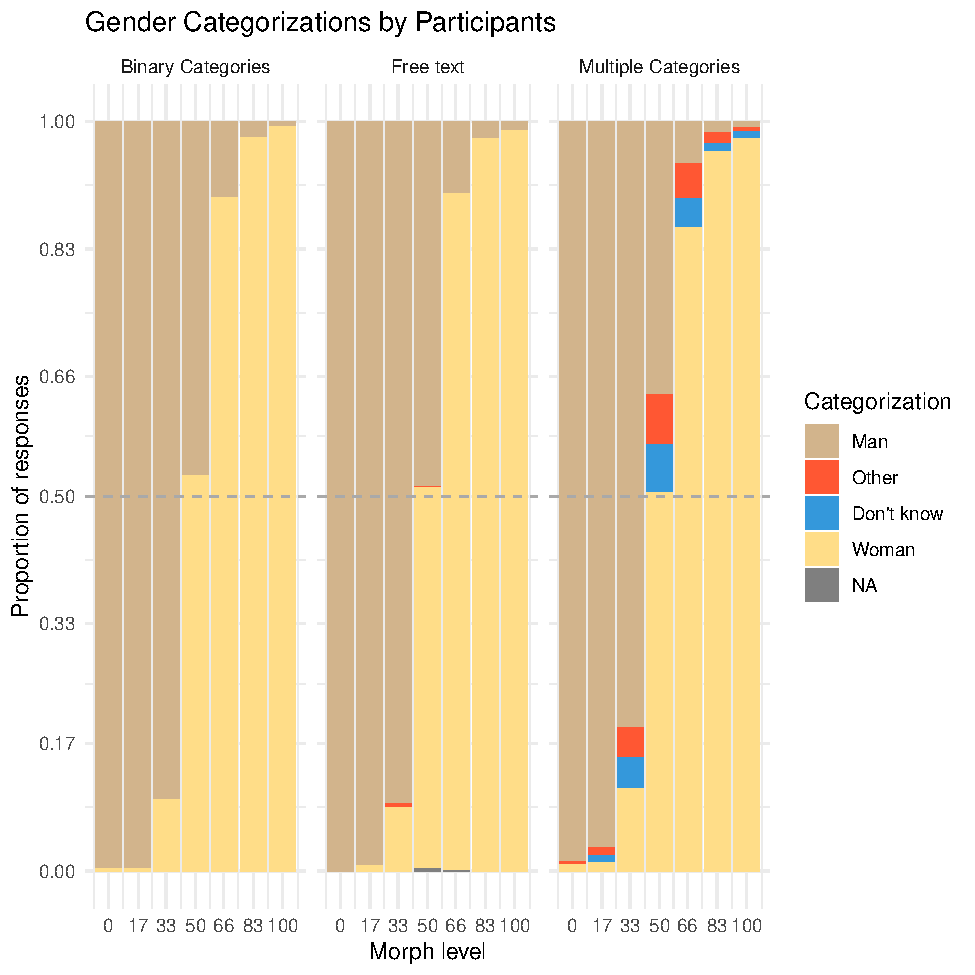
\includegraphics{quarto_test_files/figure-pdf/label - fig-descriptives-1fig.cap- Gender Categorizations by Participants-1.pdf}

There was a very clear difference between conditions; which is visible
in fig-descriptives-nbo. Figure four illustrates how many
categorizations beyond the binary participants made. Each dot represents
one participant, red dots represent the number of ``other''
categorizations made by one participant and blue dots represent the
number of ``Don't know'' responses. Grey dots represent participants who
only categorized faces as women or men. In the Free Text condition, only
two participants made any other categorization than woman and man,
whereas more than half did so in the Multiple Categories condition (see
fig-descriptives-nbo).

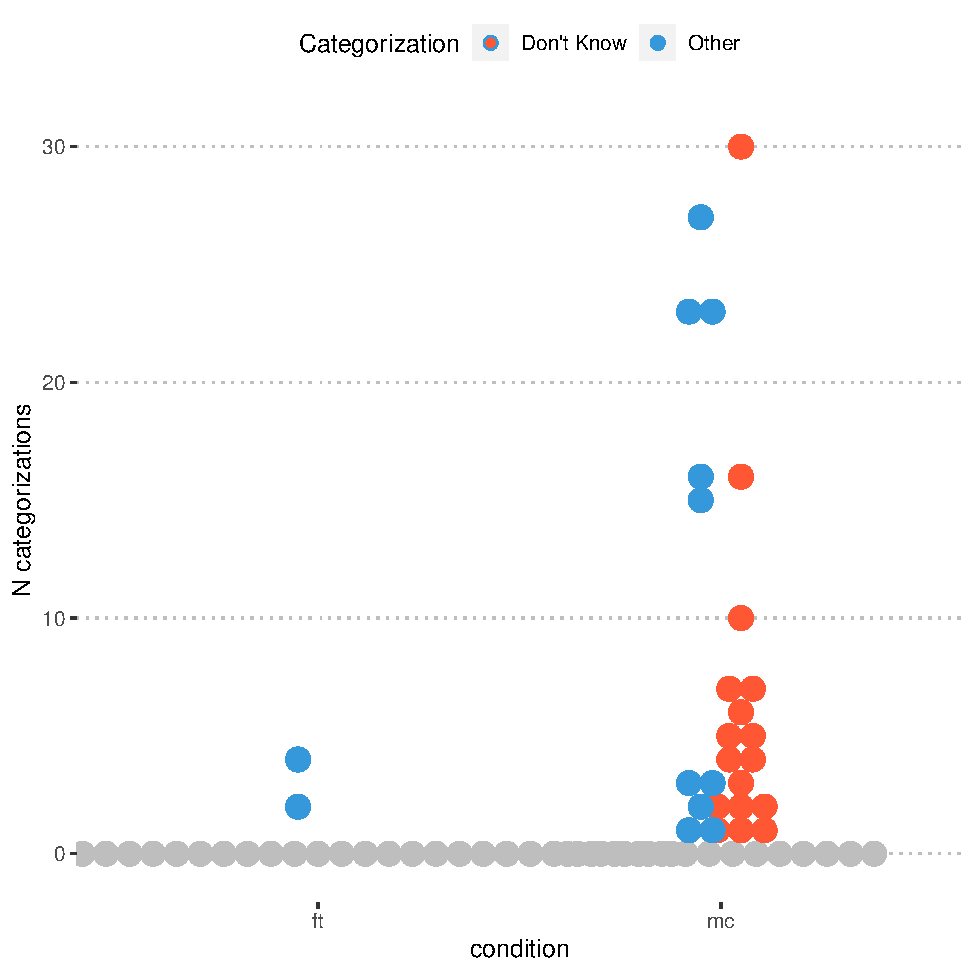
\includegraphics{quarto_test_files/figure-pdf/label - fig-descriptives-nbofig.cap- Responses of other and I don't know across the multiple categories and free text condiitons-1.pdf}

\begin{verbatim}
`summarise()` has grouped output by 'id'. You can override using the `.groups`
argument.
\end{verbatim}

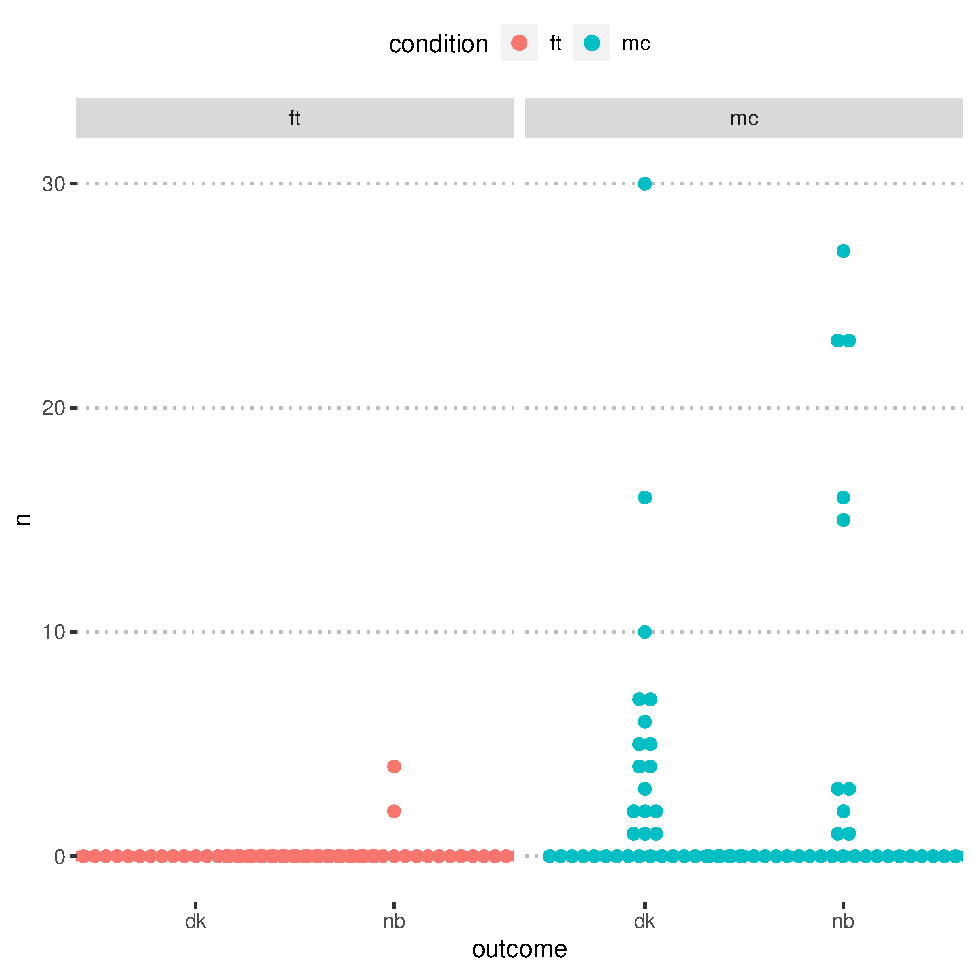
\includegraphics{quarto_test_files/figure-pdf/unnamed-chunk-10-1.pdf}

\subsubsection{Categorization within the
binary}\label{categorization-within-the-binary}

When people categorize faces beyond the binary such categorization also
affects the categorization of faces as men or women. For example, the
categorization of faces as non-binary could theoretically decrease
either ``woman'' or ``man'' categorization, if for example ``other''
categorizations consistently replaced ``woman'' categorization. We
therefore investigated how inclusive response options changed
participants' binary categorizations.

\begin{figure}[H]

\caption{Distribution of Participant Proportions for Categorizing Faces
as Women Across Three Conditions}

{\centering 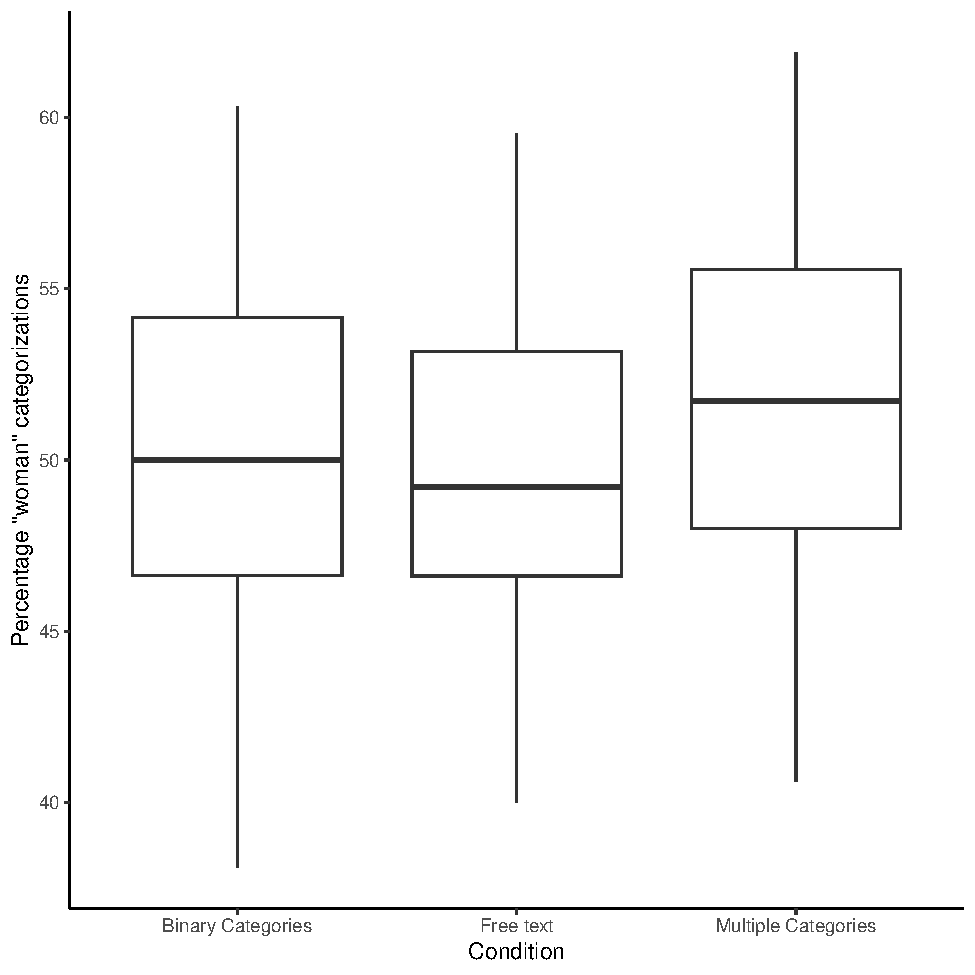
\includegraphics{quarto_test_files/figure-pdf/my-plot-1.pdf}

}

\end{figure}%

We treated the binary categories condition as a neutral baseline against
which the other two conditions were tested. The evidence indicated that
faces were categorized as women and at equal rates in the Multiple
Categories and Binary Categories conditions (OR = 0.68, CI ={[}0.4,
1.17{]}, BF\textsubscript{01}= 6.07, corresponding to moderate
evidence). The evidence also indicated that faces were categorized as
women and men at equal rates the Free text and Binary Categories
condition (OR = 1.03, CI ={[}0.6, 1.78{]}, BF\textsubscript{01}= 15.58).
In other words, neither the free text nor the multiple categories
condition changed the pattern of categorization of women and men
compared to the binary categories condition.

We also compared the relationship between facial gender and binary
categorization (i.e.~the slope of facial gender) across the conditions.
The slope of facial gender on binary categorizations was almost the same
in the multiple categories and binary categories conditions (Difference
= 0, CI ={[}-0.02, 0.03{]}, BF\textsubscript{01}= 394.93). The effect of
facial femininity on woman categorizations almost was the same in the
free text and binary categories (Difference \textgreater{} 0.001, CI
={[}-0.02, 0.02{]}, BF\textsubscript{01}= 394.93).

\subsection{Discussion}\label{discussion-1}

Experiment 2 indicated that participants categorize beyond the binary
when response options include more options than women and men only.
However, the free text option did not differ from the binary option.
Thus, the multiple categories condition, with its explicitly stated
non-binary options seems to act as reminders to participants.
Furthermore, categorization within the binary was not skewed by the
addition of multiple categories or the free text option, meaning that
the ratio of women and men categorizations was still about 50/50. This
did not systematically affect their overall pattern of responses in
terms of woman and man categorizations.

\section{General Discussion}\label{general-discussion}

In two experiments we tested how different response options influenced
gender categorization. In Study 1 we compared two-dimensional scales
with one-dimensional controls. We found that participants responded
categorically and this was the case in both the control condition and
the two-dimensional condition. In Study 2, we compared free text and
multiple categories. We found that only multiple categories elicited
beyond-binary responses. Compared to binary control, neither changed the
pattern of categorizations of women and men.

The results are consistent with previous work on categorical perception
of gender in faces(Campanella et al., 2001, 2003). Participants
exhibited a categorical pattern of responses where ratings of gender
were accentuated compared to the facial gender of the faces, suggesting
that they had a strong impression of gender as consisting of two
distinct categories. Furthermore, the two-dimensional ratings did not
reduce the strength of the categorical effect. This suggests that at
least in the present sample, two-dimensional response options were not
enough to reduce the binary gender norms.

This differs slightly from the results of Bem (1974) who found that
measuring gender as two separate scales led participants to treat gender
as less binary. Moreover, where she found that masculinity and
femininity were largely unrelated, we found that ratings of ``woman''
and ``man'' were strongly correlated. This is probably accounted for by
the differences in outcome measures. Bem (1974) measured gender as a
psychological trait in the self, whereas we measured gender as a
judgment of the physical features of others. Judging physical properties
is much more influenced by external stuff.

The finding that participants use non-binary response options is
consistent with the work of Saperstein and Westbrook (2021) and
Lindqvist et al. (2020), which has shown that including flexible
response options allows participants to better express themselves. A
recommendation from that literature is that open text boxes afford
participants the greatest flexibility in their responses. In our study,
however, that flexibility was rarely used when the response options
consisted of a free text. This likely reflects the difference between
TGD people categorizing their own gender and cisgender participants
categorizing others.

A probable explanation for the difference between free text and multiple
categories is that the multiple categories served as a visual reminder
of non-binary identity. Researchers interested in the categorization of
non-binary identity should be aware that these may not spring to mind
unless participants are explicitly reminded of them.

Neither free text nor multiple categories impacted the categorizations
of women and men. This suggests that such inclusive response options can
be suitable for investigating the categorization of women and men
without skewing the results or introducing noise. This is a positive
finding for researchers who are primarily interested in such
categorizations but do not want to contribute to the marginalization of
trans and non-binary individuals.

Overall, we recommend researchers to carefully consider how they measure
the categorization of others. Multiple dimensions, free text, and
multiple categories and continua are all viable alternatives. If the
primary research question is to investigate non-binary categorization,
then multiple categories are most suitable. However, if the goal is to
measure the categorization of women and men, free text or multiple
categories may be equally suitable.

\paragraph{Conclusion.}\label{conclusion}

In two experiments we tested how different response alternatives
affected gender categorizations. Participants were more likely to
categorize faces beyond the binary when using multiple categories,
including ``non-binary'' and ``I don't know'' than when using a free
text option. In comparison to self-identification questions where
open-ended responses are seen as the most inclusive alternative
(Lindqvist et al., 2020), the categorization of others benefits from
response options that explicitly remind participants that not all people
identify as women or men.

\newpage

\section{References}\label{references}

\phantomsection\label{refs}
\begin{CSLReferences}{1}{0}
\bibitem[\citeproctext]{ref-ansaraMethodologiesMisgenderingRecommendations2014}
Ansara, Y. G., \& Hegarty, P. (2014). Methodologies of misgendering:
{Recommendations} for reducing cisgenderism in psychological research.
\emph{Feminism \& Psychology}, \emph{24}(2), 259--270.
\url{https://doi.org/10.1177/0959353514526217}

\bibitem[\citeproctext]{ref-R-papaja}
Aust, F., \& Barth, M. (2022). \emph{{papaja}: {Prepare} reproducible
{APA} journal articles with {R Markdown}}.
\url{https://github.com/crsh/papaja}

\bibitem[\citeproctext]{ref-bemMEASUREMENTPSYCHOLOGICALANDROGYNY1974}
Bem, S. L. (1974). \emph{{THE MEASUREMENT OF PSYCHOLOGICAL ANDROGYNY}}.
8.

\bibitem[\citeproctext]{ref-R-brms_a}
Bürkner, P.-C. (2017). {brms}: An {R} package for {Bayesian} multilevel
models using {Stan}. \emph{Journal of Statistical Software},
\emph{80}(1), 1--28. \url{https://doi.org/10.18637/jss.v080.i01}

\bibitem[\citeproctext]{ref-R-brms_b}
Bürkner, P.-C. (2018). Advanced {Bayesian} multilevel modeling with the
{R} package {brms}. \emph{The R Journal}, \emph{10}(1), 395--411.
\url{https://doi.org/10.32614/RJ-2018-017}

\bibitem[\citeproctext]{ref-R-brms_c}
Bürkner, P.-C. (2021). Bayesian item response modeling in {R} with
{brms} and {Stan}. \emph{Journal of Statistical Software},
\emph{100}(5), 1--54. \url{https://doi.org/10.18637/jss.v100.i05}

\bibitem[\citeproctext]{ref-butlerGenderTroubleFeminism1999}
Butler, J. (1999). \emph{Gender trouble: Feminism and the subversion of
identity}. {Routledge}.

\bibitem[\citeproctext]{ref-campanellaCategoricalPerceptionFacial2001}
Campanella, S., Chrysochoos, A., \& Bruyer, R. (2001). Categorical
perception of facial gender information: {Behavioural} evidence and the
face-space metaphor. \emph{Visual Cognition}, \emph{8}(2), 237--262.
\url{https://doi.org/10.1080/13506280042000072}

\bibitem[\citeproctext]{ref-campanellaCategoricalPerceptionUnfamiliar2003}
Campanella, S., Hanoteau, C., Seron, X., Joassin, F., \& Bruyer, R.
(2003). Categorical perception of unfamiliar facial identities, the
face-space metaphor, and the morphing technique. \emph{Visual
Cognition}, \emph{10}(2), 129--156.
\url{https://doi.org/10.1080/713756676}

\bibitem[\citeproctext]{ref-carletonAssessingImpactRoyal2022}
Carleton, R. N., McCarron, M., Krätzig, G. P., Sauer-Zavala, S., Neary,
J. P., Lix, L. M., Fletcher, A. J., Camp, R. D., Shields, R. E.,
Jamshidi, L., Nisbet, J., Maguire, K. Q., MacPhee, R. S., Afifi, T. O.,
Jones, N. A., Martin, R. R., Sareen, J., Brunet, A., Beshai, S.,
\ldots{} Asmundson, G. J. G. (2022). Assessing the impact of the {Royal
Canadian Mounted Police} ({RCMP}) protocol and {Emotional Resilience
Skills Training} ({ERST}) among diverse public safety personnel.
\emph{BMC Psychology}, \emph{10}(1), 295.
\url{https://doi.org/10.1186/s40359-022-00989-0}

\bibitem[\citeproctext]{ref-croninYoungerGenerationsAre2022}
Cronin, K. A., Leahy, M., Ross, S. R., Wilder Schook, M., Ferrie, G. M.,
\& Alba, A. C. (2022). Younger generations are more interested than
older generations in having non-domesticated animals as pets. \emph{PLOS
ONE}, \emph{17}(1), e0262208.
\url{https://doi.org/10.1371/journal.pone.0262208}

\bibitem[\citeproctext]{ref-dagostinoOrganizationalPracticesSecondGeneration2022}
D'Agostino, M., Levine, H., Sabharwal, M., \& Johnson-Manning, A. C.
(2022). Organizational {Practices} and {Second-Generation Gender Bias}:
{A Qualitative Inquiry} into the {Career Progression} of {U}.{S}.
{State-Level Managers}. \emph{The American Review of Public
Administration}, \emph{52}(5), 335--350.
\url{https://doi.org/10.1177/02750740221086605}

\bibitem[\citeproctext]{ref-debruineWebMorph2018}
DeBruine, L. (2018). {WebMorph}. In \emph{WebMorph}.
https://webmorph.org/.

\bibitem[\citeproctext]{ref-debruineFaceResearchLab2017}
DeBruine, L. M., \& Jones, B. C. (2017). Face {Research Lab London Set}.
\emph{Figshare}. \url{https://doi.org/10.6084/m9.figshare.5047666}

\bibitem[\citeproctext]{ref-habibiSpontaneousGenderCategorization2012}
Habibi, R., \& Khurana, B. (2012). Spontaneous {Gender Categorization}
in {Masking} and {Priming Studies}: {Key} for {Distinguishing Jane} from
{John Doe} but {Not Madonna} from {Sinatra}. \emph{PLoS ONE},
\emph{7}(2), e32377. \url{https://doi.org/10.1371/journal.pone.0032377}

\bibitem[\citeproctext]{ref-hydeFutureSexGender2018}
Hyde, J. S., Bigler, R. S., Joel, D., Tate, C. C., \& van Anders, S. M.
(2018). The future of sex and gender in psychology: {Five} challenges to
the gender binary. \emph{American Psychologist}.
\url{https://doi.org/10.1037/amp0000307}

\bibitem[\citeproctext]{ref-jungAutomaticityGenderCategorization2019}
Jung, K. H., White, K. R. G., \& Powanda, S. J. (2019). Automaticity of
{Gender Categorization}: {A Test} of the {Efficiency Feature}.
\emph{Social Cognition}, \emph{37}(2), 122--144.
\url{https://doi.org/10.1521/soco.2019.37.2.122}

\bibitem[\citeproctext]{ref-levittBeingTransgenderExperience2014}
Levitt, H. M., \& Ippolito, M. R. (2014). Being {Transgender}: {The
Experience} of {Transgender Identity Development}. \emph{Journal of
Homosexuality}, \emph{61}(12), 1727--1758.
\url{https://doi.org/10.1080/00918369.2014.951262}

\bibitem[\citeproctext]{ref-lindqvistWhatGenderAnyway2020}
Lindqvist, A., Sendén, M. G., \& Renström, E. A. (2020). What is gender,
anyway: A review of the options for operationalising gender.
\emph{Psychology \& Sexuality}, 1--13.
\url{https://doi.org/10.1080/19419899.2020.1729844}

\bibitem[\citeproctext]{ref-littleRoleMasculinityDistinctiveness2002}
Little, A. C., \& Hancock, P. J. B. (2002). The role of masculinity and
distinctiveness in judgments of human male facial attractiveness.
\emph{British Journal of Psychology}, \emph{93}(4), 451--464.
\url{https://doi.org/10.1348/000712602761381349}

\bibitem[\citeproctext]{ref-maChicagoFaceDatabase2015}
Ma, D. S., Correll, J., \& Wittenbrink, B. (2015). The {Chicago} face
database: {A} free stimulus set of faces and norming data.
\emph{Behavior Research Methods}, \emph{47}(4), 1122--1135.
\url{https://doi.org/10.3758/s13428-014-0532-5}

\bibitem[\citeproctext]{ref-monroNonbinaryGenderqueerOverview2019}
Monro, S. (2019). Non-binary and genderqueer: {An} overview of the
field. \emph{International Journal of Transgenderism}, \emph{20}(2-3),
126--131. \url{https://doi.org/10.1080/15532739.2018.1538841}

\bibitem[\citeproctext]{ref-morgenrothGenderTroubleSocial2018}
Morgenroth, T., \& Ryan, M. K. (2018). Gender {Trouble} in {Social
Psychology}: {How Can Butler}'s {Work Inform Experimental Social
Psychologists}' {Conceptualization} of {Gender}? \emph{Frontiers in
Psychology}, \emph{9}. \url{https://doi.org/10.3389/fpsyg.2018.01320}

\bibitem[\citeproctext]{ref-nicholsGoodSubjectEffectInvestigating2008}
Nichols, A. L., \& Maner, J. K. (2008). The {Good-Subject Effect}:
{Investigating Participant Demand Characteristics}. \emph{The Journal of
General Psychology}, \emph{135}(2), 151--166.
\url{https://doi.org/10.3200/GENP.135.2.151-166}

\bibitem[\citeproctext]{ref-otoolePerceptionFaceGender1998}
O'Toole, A. J., Deffenbacher, K. A., Valentin, D., McKee, K., Huff, D.,
\& Abdi, H. (1998). The perception of face gender: {The} role of
stimulus structure in recognition and classification. \emph{Memory \&
Cognition}, \emph{26}(1), 146--160.
\url{https://doi.org/10.3758/BF03211378}

\bibitem[\citeproctext]{ref-R-base}
R Core Team. (2022). \emph{R: A language and environment for statistical
computing}. R Foundation for Statistical Computing.
\url{https://www.R-project.org/}

\bibitem[\citeproctext]{ref-richardsNonbinaryGenderqueerGenders2016}
Richards, C., Bouman, W. P., Seal, L., Barker, M. J., Nieder, T. O., \&
T'Sjoen, G. (2016). Non-binary or genderqueer genders. \emph{Int Rev
Psychiatry .}, \emph{28(1)}, 95--102.

\bibitem[\citeproctext]{ref-sapersteinCategoricalGradationalAlternative2021}
Saperstein, A., \& Westbrook, L. (2021). Categorical and gradational:
Alternative survey measures of sex and gender. \emph{European Journal of
Politics and Gender}, \emph{4}(1), 11--30.
\url{https://doi.org/10.1332/251510820X15995647280686}

\bibitem[\citeproctext]{ref-simanovaLinguisticPriorsShape2016}
Simanova, I., Francken, J. C., de Lange, F. P., \& Bekkering, H. (2016).
Linguistic priors shape categorical perception. \emph{Language,
Cognition and Neuroscience}, \emph{31}(1), 159--165.
\url{https://doi.org/10.1080/23273798.2015.1072638}

\bibitem[\citeproctext]{ref-stolierNeuralMechanismSocial2017}
Stolier, R. M., \& Freeman, J. B. (2017). A {Neural Mechanism} of
{Social Categorization}. \emph{The Journal of Neuroscience},
\emph{37}(23), 5711--5721.
\url{https://doi.org/10.1523/JNEUROSCI.3334-16.2017}

\bibitem[\citeproctext]{ref-R-tidyverse}
Wickham, H., Averick, M., Bryan, J., Chang, W., McGowan, L. D.,
François, R., Grolemund, G., Hayes, A., Henry, L., Hester, J., Kuhn, M.,
Pedersen, T. L., Miller, E., Bache, S. M., Müller, K., Ooms, J.,
Robinson, D., Seidel, D. P., Spinu, V., \ldots{} Yutani, H. (2019).
Welcome to the {tidyverse}. \emph{Journal of Open Source Software},
\emph{4}(43), 1686. \url{https://doi.org/10.21105/joss.01686}

\end{CSLReferences}






\end{document}
